%!TEX program = xelatex
\documentclass[conference]{IEEEtran}
\usepackage{polyglossia}
\setmainlanguage{brazil}
%\usepackage[utf8]{inputenc}
\usepackage{xcolor,graphicx,tikz,url}
\usepackage{listings}
\usepackage{setspace}
\usepackage{lipsum}
\usepackage{hyperref}
\usepackage{amsmath}
\usepackage{mathtools}
\usepackage{subfig}
\usepackage{enumitem}


\renewcommand{\lstlistingname}{Listagem}
\renewcommand{\refname}{Referências}
\renewcommand{\tablename}{Tabela}
\renewcommand{\figurename}{Figura}
\renewcommand{\abstractname}{Resumo}

\def\unb{\textsf{UnB}}
\def\red#1{\textcolor{red!50!black}{#1}}
\def\blue#1{\textcolor{blue!50!black}{#1}}
\def\green#1{\textcolor{green!50!black}{#1}}
\definecolor{mygreen}{RGB}{28,172,0} 
\definecolor{mylilas}{RGB}{170,55,241}


\lstset{language=Matlab,%
    %basicstyle=\color{red},
    breaklines=true,%
    morekeywords={matlab2tikz},
    basicstyle=\ttfamily\footnotesize,%\small,
    xleftmargin=\parindent,
    belowcaptionskip=1\baselineskip,
    keywordstyle=\color{blue},%
    morekeywords=[2]{1}, keywordstyle=[2]{\color{black}},
    identifierstyle=\color{black},%
    stringstyle=\color{mylilas},
    commentstyle=\color{mygreen},%
    showstringspaces=false,%without this there will be a symbol in the places where there is a space
    numbers=left,%
    numberstyle={\tiny \color{black}},% size of the numbers
    numbersep=5pt, % this defines how far the numbers are from the text
    emph=[1]{},emphstyle=[1]\color{red}, %some words to emphasise
    emph=[2]{X, Y, calculaMetodo2, calculaMetodo3, calculaMetodo4, calculaMetodo5, calculaMetodo6, calculaMetodo7, calculaMetodo8, calculaMetodo9}, emphstyle=[2]\color{red},    
}

\sloppy

\title{Análise de Complexidade dos Métodos de Interpolação Implementados em MATLAB}

\author{\IEEEauthorblockN{Sinayra Pascoal Cotts Moreira}
\IEEEauthorblockA{Departamento de Ciência da Computação\\Instituto de
  Ciências Exatas\\
Universidade de Brasília\\
Email:  sinayra@hotmail.com}
}
\begin{document} 

\maketitle

     
\begin{abstract} 
  Este artigo analisa uma aplicação onde, dada uma tabela $(x,y)$ descrita pelo usuário, retorna diferentes polinômios baseados nos métodos de Interpolação Polinomial. A análise implica em comparar a complexidade e tempo de execução de cada método implementado e concluir quais são os menos custosos computacionalmente.
\end{abstract}


\section{Introdução} \label{sec:intro}

Este trabalho visa a comparação da complexidade dos métodos \emph{Lagrange, Lagrange igualmente espaçado, Newton/Diferença Dividida, Diferença Finita Progressiva, Diferença Finita Regressiva, Spline Linear, Spline Cúbico Natural} e \emph{Spline Cúbico Extrapolado}~\cite{Fred_algonum,Pamplona_calnum}. Para esta análise, foram considerados três funções distintas, com $ n $ pontos, $ n \in [4, 170] $, com intervalo igualmente espaçado $ h = 1 $, anotando o tempo de execução de cada método para realizar todos os casos de testes. Os casos de testes são feitos criando uma nova tabela $(x,y)$ aplicando o polinômio calculado para cada valor de $x$ na tabela.

\section{Objetivos} \label{sec:objetivos}

O objetivo deste trabalho foi desenvolver uma implementação dos métodos de Interpolação Polinomial para consolidar os conhecimentos do curso Cálculo Numérico, relacionando esta implementação com a área de estudo do aluno. A área escolhida foi de Projeto e Análise de Algoritmo e a relação contruída foi de análise de complexidade de algoritmo. Além disso, o trabalho também teve como objetivo o estudo de linguagem de programação MATLAB, voltada para realização de cálculos numéricos com escrita próxima de expressões algébricas~\cite{introMatlab}, diferenciando-se de linguagens imperativas como C.

\section{Metodologia} \label{sec:metodologia}
Sejam dados $ n+1$ pontos $(x_{0}, y_{0}), (x_{1},y_{1}), ..., (x_{n}, y_{n})$, sendo $x_{i}$ distintos tais que $f(x_{i}) = y_{i}$, deseja-se construir um polinômio de grau não superior a $n$ que possua nos pontos $x_{i}$ os mesmos valores de $f(x_{i})$. Uma vez que este polinômio é único~\cite{polunico}, os métodos apresentados nesta Seção, apesar de apresentarem polinômios diferentes, são equivalentes.

Seja \emph{X} o vetor que possui os valores $x_{i}$ e \emph{Y} é o vetor que possui os valores de $f(x_{i})$.

\subsection{Lagrange} \label{subsec:lagrange}
O método de Lagrange é definido por
$$
\begin{matrix}
L_{n}(x)=\sum_{i=0}^{n}c_{i}l_{i}(x) & c_{i}= \frac{f(x_{i})}{P_{i}(x_{i})}&l_i(x)=\prod_{j=0, j \neq i}^{n}(x - x_{j})
\end{matrix}
$$

\begin{lstlisting}%
[caption={Resolução de $l_{i}(x)$. Complexidade $O(n^{2})$},label={lst:lagrange1}]
for i = 1:n
    produto = 1; %valor neutro
    for j = 1:n
        if(i ~= j)
            produto = double(produto) * (double(X(i)) - double(X(j)));
        end
    end
    l(i) = 1.0/produto; 
end
\end{lstlisting}

\begin{lstlisting}%
[caption={Resolução de $L_{n}(x)$ e de $c_{i}$. Complexidade $O(n^{2})$}, label={lst:lagrange2}]
function [y] = calculaMetodo2(X, Y, l, n, x)
    y = 0;
    for i = 1:n
        aux = Y(i) * l(i);
        for j = 1:n
            if(j ~= i)
                aux = aux * (x - X(j));
            end
        end
        y = y + aux;
    end
end
\end{lstlisting}

Analisando a complexidade da Listagem \ref{lst:lagrange1} e Listagem \ref{lst:lagrange2}, a complexidade do método de Lagrange  é $O(n^{2})$.

\subsection{Lagrange igualmente espaçado} \label{subsec:lagrange_esp}
O método de Lagrange igualmente espaçado é definido por
$$
\begin{matrix}
\bar{L_{n}}(u)=\sum_{i=0}^{n}c_{i}\bar{l_{i}}(u) & c_{i}= \frac{f(u_{i})}{P_{i}(u_{i})}&\bar{l_i(u)}=\prod_{j=0, j \neq i}^{n}(x - x_{j}) 
\\ u=\frac{x-x_{0}}{h} & & 
\end{matrix}
$$

\begin{lstlisting}%
[caption={Resolução de $\bar{l_{i}}(u)$. Complexidade $O(n^{2})$},label={lst:lagrange_esp1}]
for i = 0:n-1
    produto = 1; %valor neutro
    for j = 0:n-1
        if(i ~= j)
            prod = double(produto) * double((i - j));
        end
    end
    l(i+1) = 1.0/produto;
end
\end{lstlisting}

\begin{lstlisting}%
[caption={Resolução de $\bar{L_{n}}(x)$ e de $c_{i}$. Complexidade $O(n^{2})$}, label={lst:lagrange_esp2}]
function [y, u] = calculaMetodo3(X, Y, l, n, h, x)
    u = (x - X(1,1))/h;
    y = 0;
    for i = 1:n
        aux = Y(i) * l(i);
        for j = 0:n-1
            if(j ~= i-1)
                aux = aux * (u - j);
            end
        end
        y = y + aux;
    end
end
\end{lstlisting}
Analisando a complexidade da Listagem \ref{lst:lagrange_esp1} e Listagem \ref{lst:lagrange_esp2}, a complexidade do método de Lagrange igualmente espaçado é $O(n^{2})$.

\subsection{Newton/Diferença dividida} \label{subsec:newton}
O método de Newton é definido por:
$$
\begin{matrix*}[l]
N(x) =  & f[y_{0}] + \\ 
        & + f[y_{0}, y_{1}](x - x_{0}) +\\ 
        & + \cdots + \\ 
        & + f[y_{0}, \cdots ,y_{k}](x-x_{0})(x-x_{1})\cdots(x-x_{k-1}) 
\end{matrix*}
$$
$$
\begin{matrix*}[l]
\\f[y_{i}] &  = y_{i} \\ & i \in \left \{ 0 \cdots k  \right \}  & 
\\ & & 
\\f[y_{i}, \cdots, y_{i+j}] & = \frac{f[y_{i+1},\cdots, y_{i- j}] - f[y_{i},\cdots, y_{i+j-1}] }{x_{i+j} - x_{i}} \\ &  i \in \left \{ 0 \cdots k-j  \right \} 
\\ &  j \in \left \{ 1 \cdots k  \right \}
\end{matrix*}
$$

\begin{lstlisting}%
[caption={Resolução de {$f[y_{0},\cdots,y_{k}]$}. Complexidade $O(n^{2})$ },label={lst:newton_esp1}]
function [D] = f(X, Y, n, total)
    D = [];
    if(n ~= 0)
        ordem = zeros(1, n-1);
        for i = 1:n-1
            aux = (double(Y(i+1)) - double(Y(i)))/(double(X(i+1+(total-n))) - double(X(i)));
            ordem(i) = aux;
        end
        D = f(X, ordem, n-1, total); %chama f para próxima ordem, que terá n-1 elementos
        mzero = zeros(1, total - n); %ajusta para matrizes terem o mesmo tamanho
        D = [D ; Y mzero]; %concatena na resposta tudo o que encontrou
    end
end
\end{lstlisting}

\begin{lstlisting}%
[caption={Resolução de $N(x)$. Complexidade $O(n^{2})$},label={lst:newton_esp2}]
function [y] = calculaMetodo4(D, X, n, x)
    y = 0;
    for i = 1:n
        aux = D(n-(i-1), 1);
        for j = 1:i-1
            aux = aux * (x - X(j));
        end
        y = y + aux;
    end
end
\end{lstlisting}
Analisando a complexidade da Listagem \ref{lst:newton_esp1} e Listagem \ref{lst:newton_esp2}, a complexidade do método de Newton é $O(n^{2})$.

\subsection{Diferença Finita Progressiva} \label{subsec:difprog}
O método de Diferença Finita Progressiva é definido por
\begin{equation}
N_{k}(x) = \sum_{i=0}^{k}\frac{\bigtriangleup^{i}}{i!h^{i}} \prod_{j=0}^{i-1}(x-x_{j})
\end{equation}

\begin{lstlisting}%
[caption={Resolução de $\bigtriangleup^{j}$. Complexidade $O(n^{2})$ },label={lst:difprog_esp1}]
function [D] = f(Y, n, total)
    D = [];
    if(n ~= 0)
        ordem = zeros(1, n-1);
        for i = 1:n-1
            aux = double(Y(i+1)) - double(Y(i));
            ordem(i) = aux;
        end
        D = f(ordem, n-1, total); %chama f para próxima ordem, que terá n-1 elementos
        mzero = zeros(1, total - n); %ajusta para matrizes terem o mesmo tamanho
        D = [D ; Y mzero]; %concatena na resposta tudo o que encontrou
    end
end
\end{lstlisting}
\begin{lstlisting}%
[caption={Resolução de $N_{k}(x)$. Complexidade $O(n^{2})$},label={lst:difprog_esp2}]
function [y] = calculaMetodo5(D, X, h, n, x)
    y = 0;
    for i = 1:n
        d = D(n-(i-1), 1) * 1/( ( fatorial(i-1) * power(h, (i-1) ) ) );

        for j = 1:i-1
            d = d * (x - X(j));
        end
        y = y + d;
    end
end
\end{lstlisting}
Analisando a complexidade da Listagem \ref{lst:difprog_esp1} e Listagem \ref{lst:difprog_esp2}, a complexidade do método de Diferença Finita Progressiva é $O(n^{2})$.

\subsection{Diferença Finita Regressiva} \label{subsec:difreg}
O método de Diferença Finita Regressiva é definido por
\begin{equation}
N_{k}(x) = \sum_{i=0}^{k}\frac{\bigtriangledown^{i}}{i!h^{i}} \prod_{j=0}^{i-1}(x-x_{j})
\end{equation}

\begin{lstlisting}%
[caption={Resolução de $\bigtriangledown^{j}$. Complexidade $O(n^{2})$ },label={lst:difreg_esp1}]
function [D] = f(Y, n, total)
    D = [];
    if(n ~= 0)
        ordem = zeros(1, n-1);
        for i = 2:n
            aux = double(Y(i)) - double(Y(i-1));
            ordem(i-1) = aux;
        end
        D = f(ordem, n-1, total); %chama f para próxima ordem, que terá n-1 elementos
        mzero = zeros(1, total - n); %ajusta para matrizes terem o mesmo tamanho
        D = [D ; Y mzero]; %concatena na resposta tudo o que encontrou
    end
end
\end{lstlisting}

\begin{lstlisting}%
[caption={Resolução de $N_{k}(x)$. Complexidade $O(n^{2})$},label={lst:difreg_esp2}]
function [y] = calculaMetodo6(D, X, h, n, x)
    y = 0;
    for i = 1:n
        d = D(n-(i-1), 1) * 1/( ( fatorial(i-1) * power(h, (i-1) ) ) );

        for j = 1:i-1
            d = d * (x - X(j));
        end
        y = y + d;
    end
end
\end{lstlisting}
Analisando a complexidade da Listagem \ref{lst:difreg_esp1} e Listagem \ref{lst:difreg_esp2}, a complexidade do método de Diferença Finita Regressiva é $O(n^{2})$.

\subsection{Spline Linear} \label{subsec:splinelinear}
O método Spline Linear, $S_{1}(x)$, tem grau $1$ e pode ser escrito em cada subintervalo $[x_{i-1}, x{i}], i \in \left \{ 0 \cdots k  \right \} $, de modo que
$$
s_{i}(x)=f(x_{i-1})\frac{x_i-x}{x_i-x_{i-1}}+f(x_{i})\frac{x-x_{i-1}}{x_i-x_{i-1}}, \forall x \in [x_{i-1},x_{i}]
$$

\begin{lstlisting}%
[caption={Limitação dos intervalos. Complexidade $O(n)$ },label={lst:splinelinear_esp1}]
for i = 1:n-1
    intervalo(i, 1) = Xi(i);
    intervalo(i, 2) = Xi(i+1);
    xs(i) = 1/(Xi(i) - Xi(i+1));
end
\end{lstlisting}

\begin{lstlisting}%
[caption={Resolução de $s_{i}$. Complexidade $O(n)$ },label={lst:splinelinear_esp2}]
function [Yf, I] = calculaMetodo7(X, Y, intervalo, xs, n, x)
    Yf = [];
    I = [];
    for i = 1:n-1
        if(x >= intervalo(i, 1) && x <= intervalo(i, 2))
            y = Y(i) * (x - X(i+1)) - Y(i+1)*(x - X(i));
            y = y * xs(i);
            Yf = [Yf y]; %y dentro do intervalo
            I = [I i]; %intervalo
        end
    end
end
\end{lstlisting}

Analisando a complexidade da Listagem \ref{lst:splinelinear_esp1} e Listagem \ref{lst:splinelinear_esp2}, a complexidade do método de Spline Linear é $O(n)$.

\subsection{Spline Cúbico Natural} \label{subsec:splinecubnat}
O método Spline Cúbico Natural, $S_{3}(x)$, tem grau $3$ e pode ser escrito em cada subintervalo $[x_{i-1}, x{i}], i \in \left \{ 0 \cdots k  \right \} $, de modo que
$$
s_{i}(x)=a_{i}(x-x_{i})^{3}+b_{i}(x-x_{i})^{2}+c_{i}(x-x_{i}) + d_{i}
$$
$$
\begin{matrix}
a_i = \frac{g_i - g_{i-1}}{6h_i} & b_i = \frac{g_i}{2} & c_i = \frac{h_i}{6}(g_{i-1}+2g_i)+f[x_{i-1}, x_i] & \\ d_i=y_i
\end{matrix}
$$
Onde
$A.\bar{g}=\bar{y}$
$$
A=\begin{pmatrix}
%2_h1 &h_1  & 0 & 0 & \cdots & 0 & 0\\ 
 h_1& 2(h_1+h_2) &h_2  &  \cdots & 0 & 0 & 0 \\ 
 \vdots  \\ 
 %0& 0 & 0 & 0 & \cdots & h_k&2h_k 
 0& 0 & 0  & \cdots & h_{k-1} & 2(h_{k-1} + h_k)&h_k 
\end{pmatrix}
$$
$$
\bar{y} = 6\begin{pmatrix}
 %f[x_0,x_1] - {y_0}'
f[x_1,x_2] - f[x_0,x_1]
\\ \vdots 
%\\{y_k}' - f[x_{k-1},x_k]
\\f[x_{k-2},x_{k-1}] - f[x_{k-1},x_k]
\end{pmatrix} 
\bar{g} = \begin{pmatrix}
 g_0
\\ g_1
\\ \vdots 
\\g_k
\end{pmatrix}
$$

\begin{lstlisting}%
[caption={Limitação dos intervalos e resolvendo matriz $\bar{y}$. Complexidade $O(n)$ },label={lst:splinecubnat_esp1}]
for i = 1:n-1
        
    intervalo(i, 1) = Xi(i);
    intervalo(i, 2) = Xi(i+1);
    hs(i) = Xi(i+1) - Xi(i);  %h
    f(i) = (Yi(i+1) - Yi(i))/hs(i); %newton
end
for i = 1:n-2
    y(i) = f(i+1) - f(i);
end
y = 6 * y; %y
\end{lstlisting}

\begin{lstlisting}%
[caption={Resolvendo matriz $A$. Complexidade $O(n)$ },label={lst:splinecubnat_esp2}]
j = -1;
for i = 1:n-2
    coluna = 1;
    
    if(j + coluna >= 1 && j + coluna <= (n-2))
        A(i, coluna+j) = hs(i);
    end
    
    coluna = coluna + 1;
    if(j + coluna >= 1 && j + coluna <= (n-2))
        A(i, coluna+j) = 2 * (hs(i) + hs(i+1));
    end
    
    coluna = coluna + 1;
    if(j + coluna >= 1 && j + coluna <= (n-2))
        A(i, coluna+j) = hs(i+1);
    end
    
    j = j + 1;
end
\end{lstlisting}

\begin{lstlisting}%
[caption={Resolvendo matriz $\bar{g}$. Complexidade $O(n^2)$ },label={lst:splinecubnat_esp3}]
g(n) = A(n,(n+1))/A(n,n);
i = n-1;        %De trás para frente
while(i >= 1)
    j = n;
    while(j > i)
        g(i) = g(i) - g(j)*A(i,j); %subtrai todos os a's que possuem valor com seus respectivos x's
        j = j - 1;
    end
    g(i) = g(i) + A(i, n+1); %soma com respectivo yi que foi triangulizado
    g(i) = g(i) / A(i,i); %divide com xi respectivo
    i = i - 1;    
end
\end{lstlisting}

\begin{lstlisting}%
[caption={Resolução de $s_i$. Complexidade $O(n)$ },label={lst:splinecubnat_esp4}]
function [Yf, I] = calculaMetodo8(X, Y, intervalo, g, h, f, n, x)
    Yf = [];
    I = [];
    for i = 2:n
        if(x >= intervalo(i-1, 1) && x <= intervalo(i-1, 2))
            a = (g(i) - g(i-1))/(6*h(i-1));
            b = g(i)/2;
            c = f(i-1) + (2*h(i-1)*g(i) + g(i-1)*h(i-1))/6;
            d = Y(i);
            y = a * power(x - X(i), 3) + b * power(x - X(i), 2) + c * (x - X(i)) + d;
            Yf = [Yf y];
            I = [I i-1];

        end
    end
end
\end{lstlisting}
Analisando a complexidade da Listagem \ref{lst:splinecubnat_esp1}, Listagem \ref{lst:splinecubnat_esp2}, Listagem \ref{lst:splinecubnat_esp3} e Listagem \ref{lst:splinecubnat_esp4}, a complexidade do método de Spline Cúbico Natural é $O(n^2)$.

\subsection{Spline Cúbico Extrapolado} \label{subsec:splinecubext}
O método Spline Cúbico Extrapolado, $S_{3}(x)$, tem grau $3$ e pode ser escrito em cada subintervalo $[x_{i-1}, x{i}], i \in \left \{ 0 \cdots k  \right \} $, de modo que
$$
s_{i}(x)=a_{i}(x-x_{i})^{3}+b_{i}(x-x_{i})^{2}+c_{i}(x-x_{i}) + d_{i}
$$
$$
\begin{matrix}
a_i = \frac{g_i - g_{i-1}}{6h_i} & b_i = \frac{g_i}{2} & c_i = \frac{h_i}{6}(g_{i-1}+2g_i)+f[x_{i-1}, x_i] & \\ d_i=y_i
\end{matrix}
$$
Onde
$A.\bar{g}=\bar{y}$
$$
A=\begin{pmatrix}
2_h1 &h_1  & 0 & 0 & \cdots & 0 & 0\\ 
 h_1& 2(h_1+h_2) &h_2  & 0 & \cdots & 0 & 0 \\ 
 0 &  h_2& 2(h_2+h_3) &h_3  & \cdots &0 & 0 \\ 
 \vdots  \\ 
 0& 0 & 0 & 0 & \cdots & h_k&2h_k 
\end{pmatrix}
$$
$$
\bar{y} = 6\begin{pmatrix}
 f[x_0,x_1] - {y_0}'
\\ f[x_1,x_2] - f[x_0,x_1]
\\ \vdots 
\\{y_k}' - f[x_{k-1},x_k]
\end{pmatrix} 
\bar{g} = \begin{pmatrix}
 g_0
\\ g_1
\\ \vdots 
\\g_k
\end{pmatrix}
$$

\begin{lstlisting}%
[caption={Limitação dos intervalos e resolvendo matriz $\bar{y}$. Complexidade $O(n)$.},label={lst:splinecubext_esp1}]
%ajustando h e calculando f(newton)
f(1) = y0; %derivada de f(x) usando x0
for i = 1:n-1
    intervalo(i, 1) = Xi(i);
    intervalo(i, 2) = Xi(i+1);
    h(i) = Xi(i+1) - Xi(i);
    f(i+1) = (Yi(i+1) - Yi(i))/h(i);

end
hs = [0 h 0];
f(n+1) = yn; %derivada de f(x) usando xn
%ajustando y
for i = 1:n
    y(i) = f(i+1) - f(i);
end
y = 6 * y;
\end{lstlisting}

\begin{lstlisting}%
[caption={Resolvendo matriz $A$. Complexidade $O(n)$.},label={lst:splinecubext_esp2}]
%ajustando A
j = -1;
for i = 1:n
    coluna = 1;

    if(j + coluna >= 1 && j + coluna <= (n))
        A(i, coluna+j) = hs(i);
    end
    
    coluna = coluna + 1;
    if(j + coluna >= 1 && j + coluna <= (n))
        A(i, coluna+j) = 2 * (hs(i) + hs(i+1));
    end
    
    coluna = coluna + 1;
    if(j + coluna >= 1 && j + coluna <= (n))
        A(i, coluna+j) = hs(i+1);
    end
    
    j = j + 1;
end
\end{lstlisting}

\begin{lstlisting}%
[caption={Resolvendo matriz $\bar{g}$. Complexidade $O(n^2)$ },label={lst:splinecubext_esp3}]
g(n) = A(n,(n+1))/A(n,n);
i = n-1;        %De trás para frente
while(i >= 1)
    j = n;
    while(j > i)
        g(i) = g(i) - g(j)*A(i,j); %subtrai todos os a's que possuem valor com seus respectivos x's
        j = j - 1;
    end
    g(i) = g(i) + A(i, n+1); %soma com respectivo yi que foi triangulizado
    g(i) = g(i) / A(i,i); %divide com xi respectivo
    i = i - 1;   
end
\end{lstlisting}

\begin{lstlisting}%
[caption={Resolução de $s_i$. Complexidade $O(n)$ },label={lst:splinecubext_esp4}]
function [Yf, I] = calculaMetodo9(X, Y, intervalo, g, h, f, n, x)
    Yf = [];
    I = [];
    for i = 2:n
        if(x >= intervalo(i-1, 1) && x <= intervalo(i-1, 2))
            a = (g(i) - g(i-1))/(6*h(i-1));
            b = g(i)/2;
            c = f(i) + (2*h(i-1)*g(i) + g(i-1)*h(i-1))/6;
            d = Y(i);
            y = a * power(x - X(i), 3) + b * power(x - X(i), 2) + c * (x - X(i)) + d;
            Yf = [Yf y];
            I = [I i-1];
        end
    end
end
\end{lstlisting}

Analisando a complexidade da Listagem \ref{lst:splinecubext_esp1}, Listagem \ref{lst:splinecubext_esp2}, Listagem \ref{lst:splinecubext_esp3} e Listagem \ref{lst:splinecubext_esp4}, a complexidade do método de Spline Cúbico Extrapolado é $O(n^2)$.
\section{Desenvolvimento}\label{sec:desenvolvimento}

Ao iniciar a aplicação, o programa realiza uma série de perguntas ao usuário para montar a tabela $(x,y)$. Dentre as perguntas, estão se o usuário irá escrever uma função (ou se irá apenas digitar os valores na tabela), se será igualmente espaçada e se deseja ser informado sobre o progresso dos cálculos que serão realizados durante a execução da aplicação. Após isso, o programa inseres os valores caso não estejam na tabela, verifica se os valores de $x$ estão ordenados e se os pares $(x,y)$ caracterizam uma função. Em seguida, o programa oferece uma lista de métodos (explicados na Seção \ref{sec:metodologia}) que podem ser aplicados. Com o método escolhido pelo usuário, o programa imprime na tela o polinômio correspondente e oferece a opção de testar ou interpolar o polinômio. Cada método foi desenvolvido em um arquivo separado do programa principal.

No caso da análise de complexidade de cada método, foi criado uma versão automatizada do mesmo programa, sendo que este não realiza operações de entrada e saída na tela. O tempo analisado foi somente do tempo total de realização dos testes de cada polinômio, não sendo considerado os erros acumulados de cada teste. 

Na escolha de quantidade de pontos, foi considerado a maior quantidade de pontos que não causasse \emph{overflow} nem \emph{underflow} em nenhum dos métodos analisados. Uma vez que os métodos de Diferenças Finitas \ref{subsec:difprog} \ref{subsec:difreg} utilizam a operação \emph{fatorial} e o fatorial do MATLAB possui fator de saturação para dados do tipo \emph{double} de \emph{171} \cite{fac}, o intervalo escolhido para análise foi de $x \in \left \{ 4 \cdots 171  \right \}$.
\subsection{Especificações} \label{subsec:espec}
\begin{itemize}[leftmargin=23.5mm]
  \item [Software] MATLAB R2015b
  \item [Workspace]
    \begin{itemize}
      \item Windows 10;
      \item 12GB de memória RAM;
      \item Processador Intel i3 3.5GHz;
    \end{itemize}
  
\end{itemize}

\section{Resultados} \label{sec:resultados}
Na Figura \ref{fig:tempo-abs} é apresentado os tempos absolutos por quantidade de pontos, na Figura \ref{fig:tempo-log10} é aplicada escala logarítima no tempo de execução dos testes e na Figura \ref{fig:tempo-loglog10} é aplicada escala logarítima em ambos os eixos.
\begin{figure}[t]
  \subfloat[$f(x) = xe^{x}$]{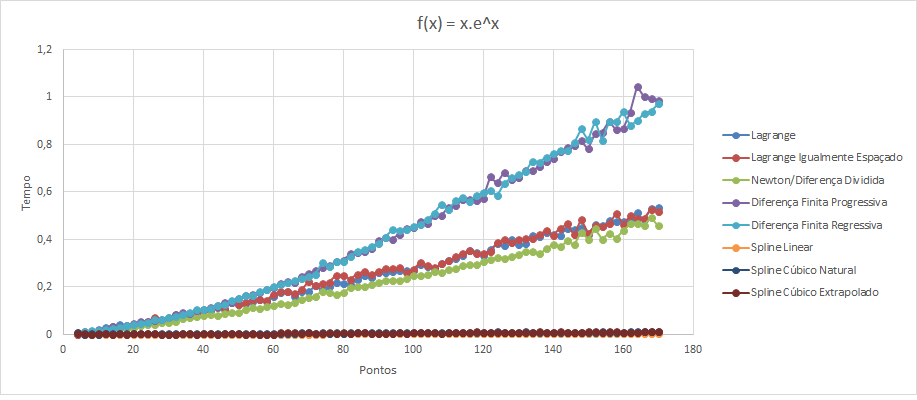
\includegraphics[width=\linewidth]{img/func1-1}\label{fig:func1-1}} \hspace{\fill}
  \subfloat[$f(x) = \frac{1}{1+x^{2}}$]{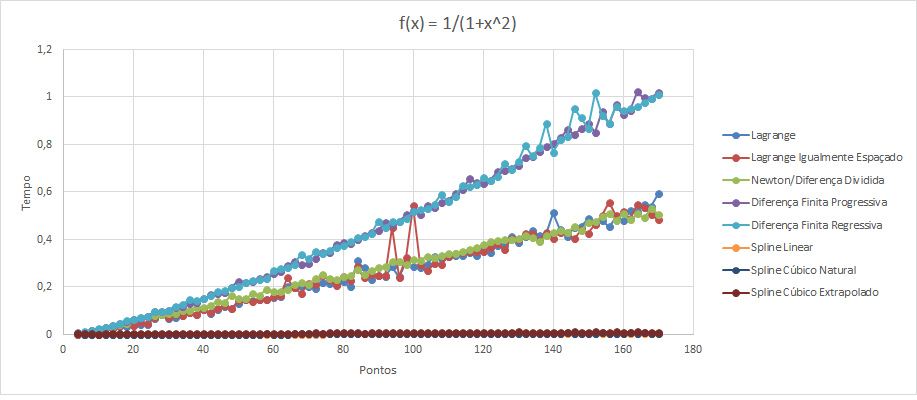
\includegraphics[width=\linewidth]{img/func2-1}\label{fig:func2-1}} \hspace{\fill}
  \subfloat[$f(x) = \cos(\pi x - \frac{\pi }{2}) $]{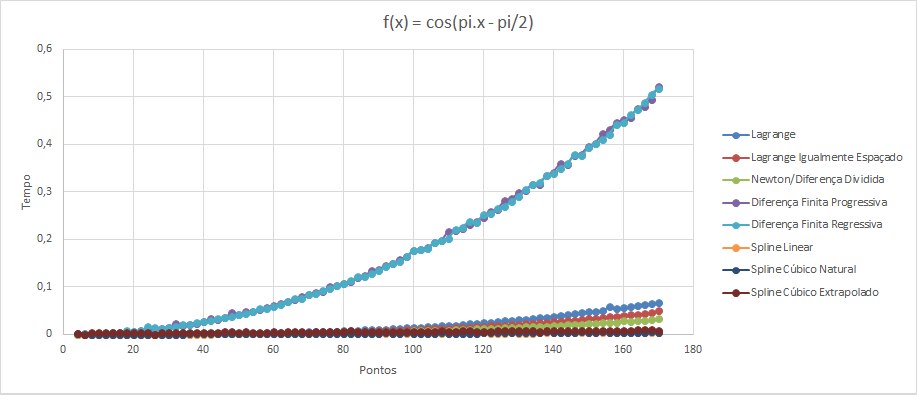
\includegraphics[width=\linewidth]{img/func3-1}\label{fig:func3-1}}
  \caption{Tempo absoluto de execução dos testes} 
  \label{fig:tempo-abs}
\end{figure}

Podemos notar, na Figura \ref{fig:tempo-abs}, que independente da função de entrada, os métodos de Diferença Finita (\ref{subsec:difprog} e \ref{subsec:difreg}) possuem o maior tempo de execução comparado com os outros métodos, e isso pode ser explicado devido a operação de \emph{fatorial}. Mesmo que os métodos explicados na Seção \ref{sec:metodologia} possuem complexidade $O(n^2)$, com exceção do método Spline Linear \ref{subsec:splinelinear}, podemos reparar a diferença que operações de soma, multiplicação e recursão causam no processamento do algoritmo, sendo que estas diferenças seriam consideradas irrelevantes caso fosse possível uma quantidade infinita de pontos para serem analisados.

\begin{figure}[t]
  \subfloat[$f(x) = xe^{x}$]{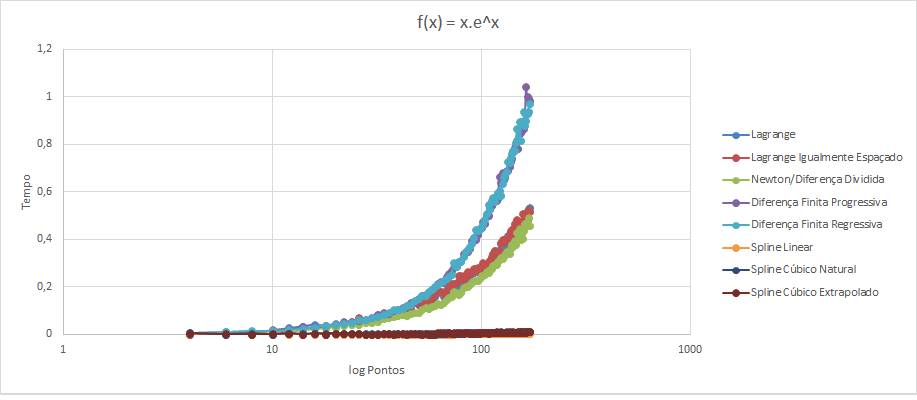
\includegraphics[width=\linewidth]{img/func1-2}\label{fig:func1-2}} \hspace{\fill}
  \subfloat[$f(x) = \frac{1}{1+x^{2}}$]{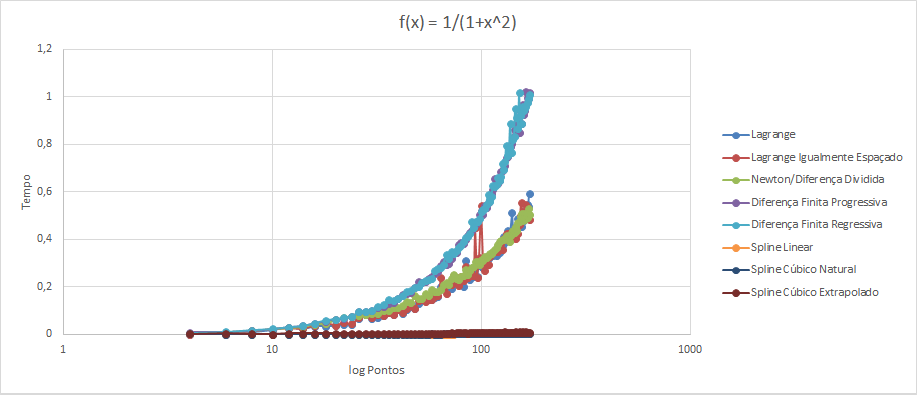
\includegraphics[width=\linewidth]{img/func2-2}\label{fig:func2-2}} \hspace{\fill}
  \subfloat[$f(x) = \cos(\pi x - \frac{\pi }{2}) $]{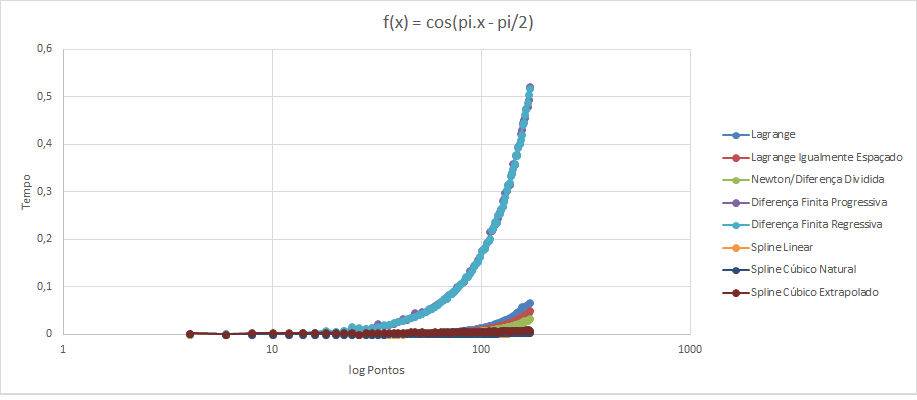
\includegraphics[width=\linewidth]{img/func3-2}\label{fig:func3-2}}
  \caption{Escala logarítima no tempo de execução} 
  \label{fig:tempo-log10}
\end{figure}

Na Figura \ref{fig:tempo-log10} fica mais explícito que os métodos estão seguindo sua complexidade descrita. Entretanto, nos métodos de Spline Cúbicos (\ref{subsec:splinecubnat} e \ref{subsec:splinecubext}) não fica tão explícito sua complexidade devido a limitação de pontos imposta pelos outros métodos. Caso fossem analisados separadamente, a quantidade de pontos máximas poderia ser ampliada para \emph{700} pontos sem causar \emph{overflow}.

\begin{figure}[t]
  \subfloat[$f(x) = xe^{x}$]{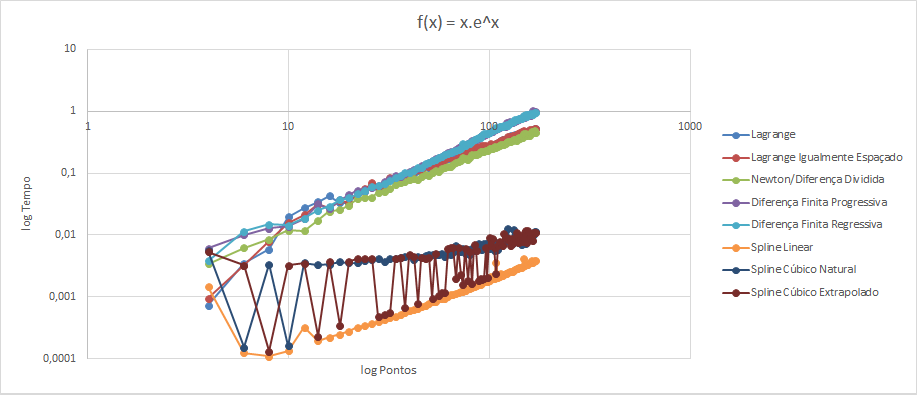
\includegraphics[width=\linewidth]{img/func1-3}\label{fig:func1-3}} \hspace{\fill}
  \subfloat[$f(x) = \frac{1}{1+x^{2}}$]{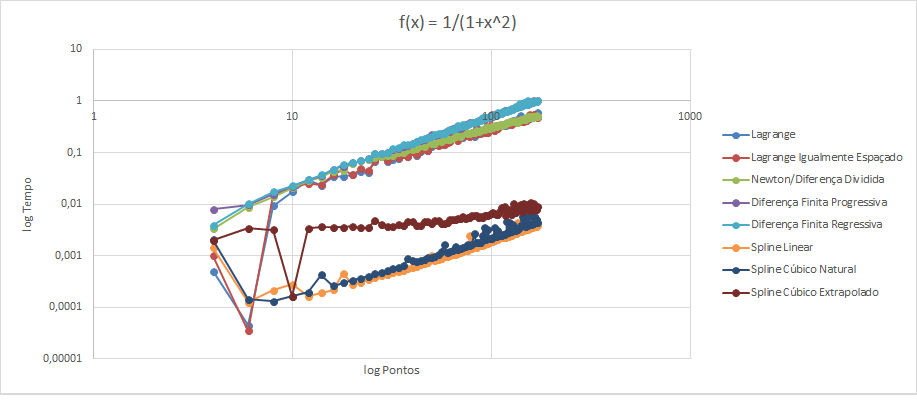
\includegraphics[width=\linewidth]{img/func2-3}\label{fig:func2-3}} \hspace{\fill}
  \subfloat[$f(x) = \cos(\pi x - \frac{\pi }{2}) $]{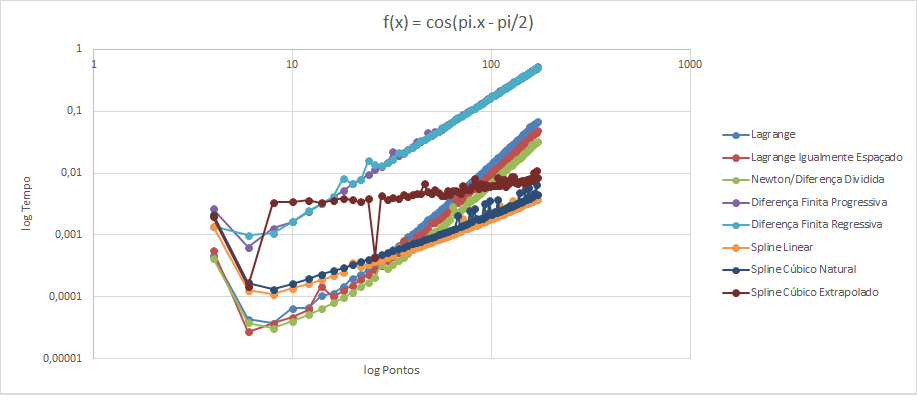
\includegraphics[width=\linewidth]{img/func3-3}\label{fig:func3-3}}
  \caption{Escala logarítima em ambos os eixos} 
  \label{fig:tempo-loglog10}
\end{figure}

Na Figura \ref{fig:tempo-loglog10} é possível visualizar o custo computacional de todos os métodos, concluindo que o método Spline Linear é o menos custoso computacionalmente se levarmos a quantidade de pontos para infinito.
\section{Trabalhos futuros} \label{sec:trabalhosfut}
Devido a limitação computacional do \emph{workspace} onde foi realizado os testes e do próprio \emph{software}, poderia ser analisado o desenvolvimento da mesma aplicação em outras linguagens matemáticas, como a linguagem R, e que os testes sejam aplicados em uma quantidade maior de computadores, preferencialmente com melhores especificações. 
Além disso, para que operações que não sejam \emph{loop} não interfiram na análise do algoritmo, é necessário uma otimização das operações realizadas por cada método, como o próprio \emph{fatorial} ou \emph{exponenciação}, com o objetivo de ser possível uma análise de maiores quantidade de pontos.

\bibliographystyle{plain}
\bibliography{sbc-template}

\end{document}
